\documentclass[final,t]{beamer}
\mode<presentation>
{
%  \usetheme{Warsaw}
%  \usetheme{Aachen}
%  \usetheme{Oldi6}
%  \usetheme{I6td}
%  \usetheme{I6dv}
%  \usetheme{I6pd}
\usepackage{verbatim}
  \usetheme{I6pd3}
% \usetheme{Icy}
}
% additional settings
%\setbeamerfont{itemize}{size=\normalsize}
%\setbeamerfont{itemize/enumerate body}{size=\normalsize}
%\setbeamerfont{itemize/enumerate subbody}{size=\normalsize}
\definecolor{StemExpansionColor}{rgb}{0.2,0.2,0.2}

% additional packages

\usepackage{wrapfig}
\usepackage{graphicx}
\usepackage{times}
\usepackage{enumerate}
%\usepackage{mdwlist}
\usepackage{amsmath,amsthm, amssymb, latexsym}
\usepackage{exscale}
%\boldmath
\usepackage{booktabs, array}
\usepackage{multirow}
%\usepackage{rotating} %sideways environment
\usepackage[english]{babel}
\usepackage[latin1]{inputenc}
\usepackage[orientation=landscape,size=custom,width=81,height=91,scale=1.0]{beamerposter}
\graphicspath{{figures/}}
% Display a grid to help align images
%\beamertemplategridbackground[1cm]

\newcommand{\Dir}{\mathrm{Dir}}
\newcommand{\Mult}{\mathrm{Mult}}
\newcommand{\expect}[1]{\mathbb{E}\left[#1\right]}
\newcommand{\transpose}[1]{{#1}^{\mathsf{T}}}

\newcommand{\partl}[2]{\frac{\partial #1}{\partial #2}}

\newcommand{\mv}{\tilde{m}} 
\newcommand{\z}{\bold{z}} 
\newcommand{\vv}[0]{\tilde{V}}
\newcommand{\W}{\textbf{W}}
\newcommand{\w}{\textbf{w}}
\newcommand{\vphi}{\phi}
\newcommand{\bv}{\tilde{\beta}}
\newcommand{\bb}{\beta}
\newcommand{\lv}{\tilde{l}}
\newcommand{\vlv}{\sigma^2_{l}}
\newcommand{\vd}{\sigma^2_{d}}
\newcommand{\vbv}{\sigma^2}
\newcommand{\stdnorm}[1]{\mathcal{N}\left(#1\right)}

\title{\Huge Modeling influence in Text Corpora}
\author[Gerrish et al.]{Sean Gerrish \hspace{2.5in}David M. Blei}
\institute[Princeton University]{Department of Computer Science}
\date[Apr. 1, 2010]{Apr 1, 2010}

% abbreviations
\usepackage{xspace}
\makeatletter
\DeclareRobustCommand\onedot{\futurelet\@let@token\@onedot}
\def\@onedot{\ifx\@let@token.\else.\null\fi\xspace}
\def\eg{{e.g}\onedot} \def\Eg{{E.g}\onedot}
\def\ie{{i.e}\onedot} \def\Ie{{I.e}\onedot}
\def\cf{{c.f}\onedot} \def\Cf{{C.f}\onedot}
\def\etc{{etc}\onedot}
\def\vs{{vs}\onedot}
\def\wrt{w.r.t\onedot}
\def\dof{d.o.f\onedot}
\def\etal{{et al}\onedot}
\makeatother

%%%%%%%%%%%%%%%%%%%%%%%%%%%%%%%%%%%%%%%%%%%%%%%%%%%%%%%%%%%%%%%%%%%%%%%%%%%%%%%%%%%%%%%%%%%%%%%%%%%%%%%%%%%%
%%%%%%%%%%%%%%%%%%%%%%%%%%%%%%%%%%%%%%%%%%%%%%%%%%%%%%%%%%%%%%%%%%%%%%%%%%%%%%%%%%%%%%%%%%%%%%%%%%%%%%%%%%%%
\begin{document}
\begin{frame}{} 

  \begin{columns}[t]
    \begin{column}{.34\linewidth}
      \begin{block}{Basic Idea}
        \hspace{-1.6cm} \parbox{.93\textwidth}{
 Identifying the most influential
documents in a corpus is an important problem in many fields, ranging
from information science and historiography to text summarization and
news aggregation. Researchers often turn to citation metrics to assess
the impact of these articles, and these approaches often work well when
citations are available.

\vspace{0.03\textwidth} However, the notion of impact or influence
transcends the presence or availability of citations.
\textbf{\textit{Our goal is to develop unsupervised methods which can
help us identify influential documents in the \textit{absence} of
highly structured information like citations.}  } Instead, we use
changes in the language of these documents over time. While we are
interested in corpora for which this information is not available, we
can (and do) use citation counts to measure our model's performance.

\begin{figure}
  \includegraphics[width=0.8\textwidth]{../figures/influence_intuition.pdf}
\end{figure}

\vspace{0.03\textwidth} Our intuition is that influential documents
change the \textit{language} of their fields of study. To formalize
this, we use ideas from the \textit{Dynamic Topic Model} (DTM), which
allows us to model topics whose language changes over time. A DTM
assumes that the topics themselves drift over time, capturing changes
in topics' language.  We assume that an influential document causes a
shift in the vocabulary of a topic, depending on the words in the
document itself and an influence variable associated with each
document.  }
\end{block}


\begin{block}{A Closer Look}
These plots show how words in documents found by our model tend to be
used more or less over time in certain topics.
\label{block:example_documents}
%\parbox{.95\textwidth}{
      \begin{figure}
      \begin{tabular}{cc}
%\.
% \hline
%      \textbf{\emph{A Maximum Entropy Model For}}
%     & \textbf{\emph{An Ascription-Based Approach}} \\
%     \textbf{\emph{Part-of-Speech Tagging (3.63)}}
%      & \textbf{\emph{To Speech Acts (-4.22)}} \\ \hline
      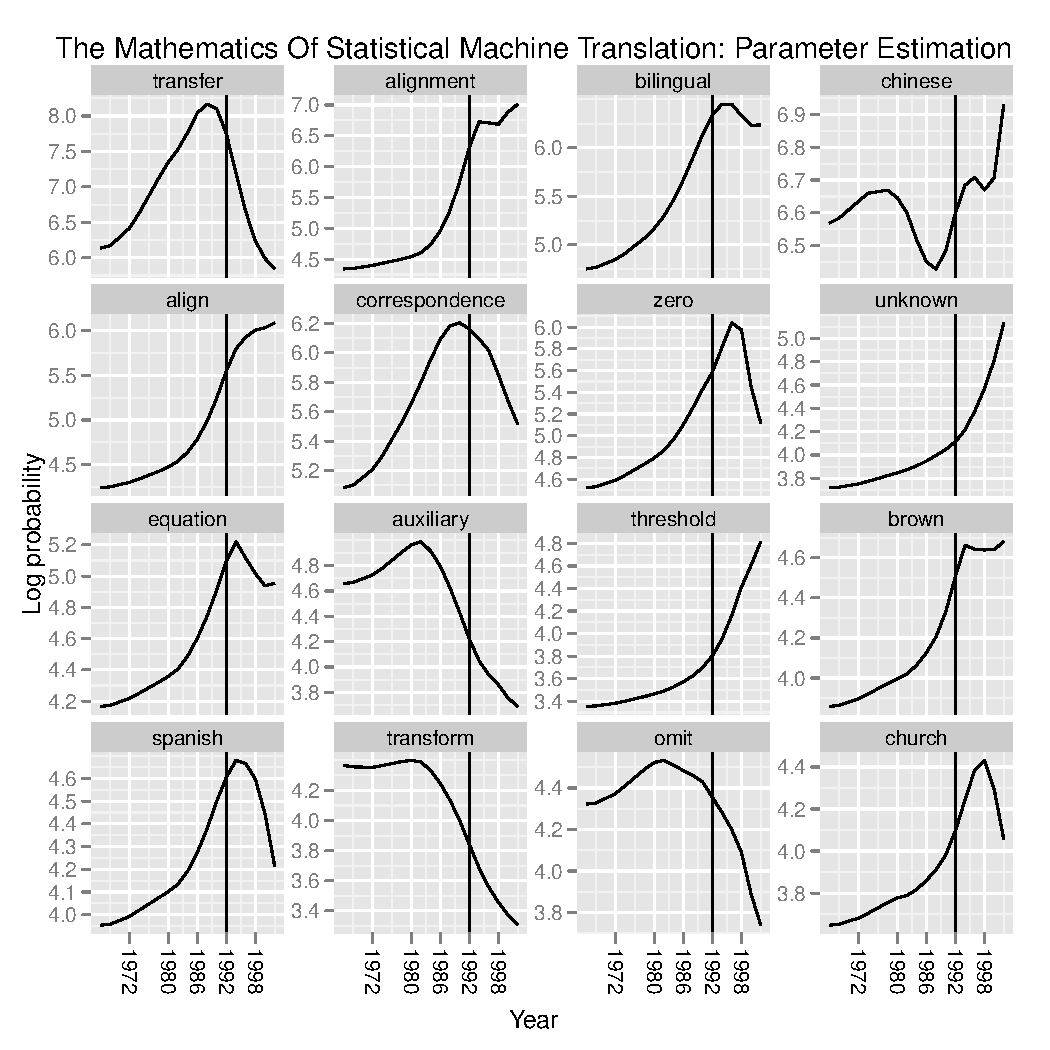
\includegraphics[width=0.4\textwidth]{../figures/acl_brown.pdf} &
      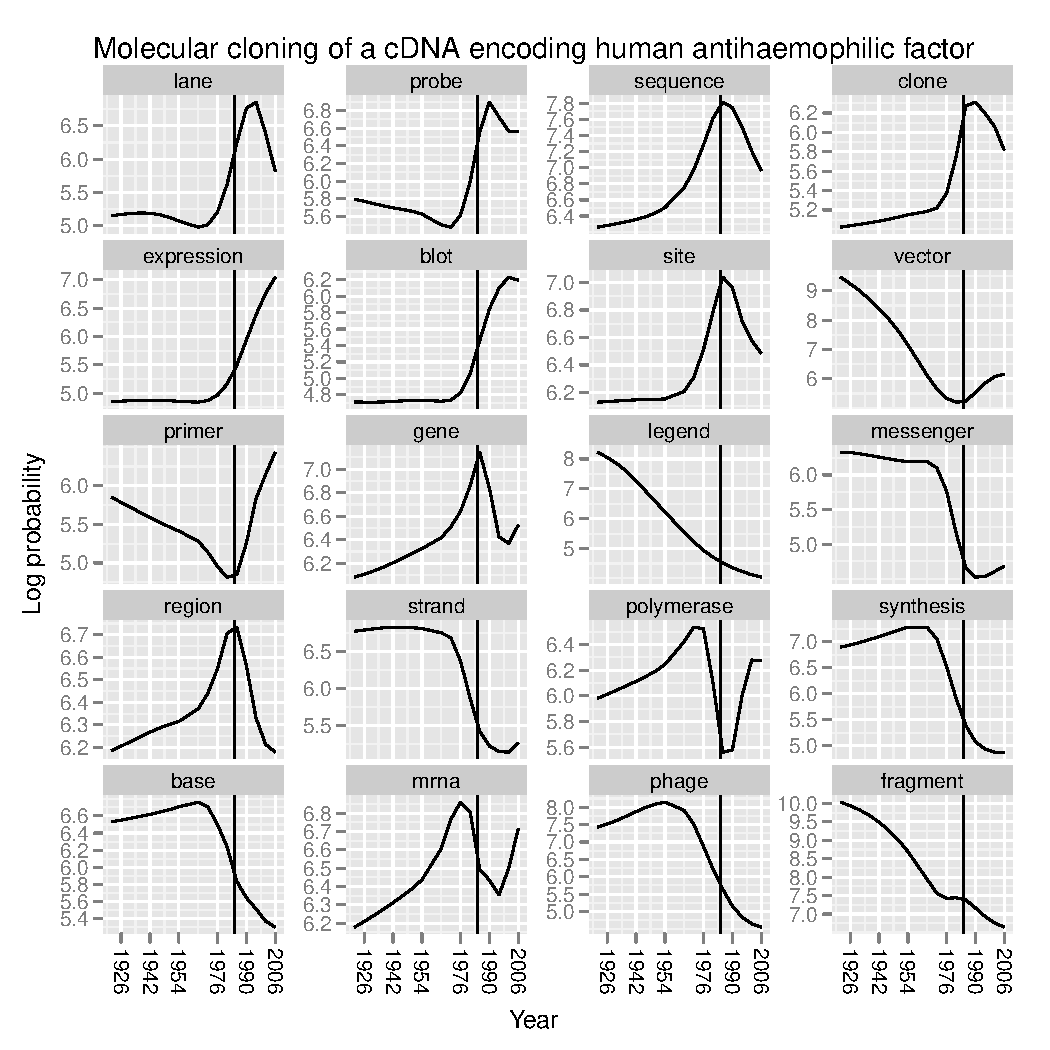
\includegraphics[width=0.4\textwidth]{../figures/nature_cloning.pdf} \\
%      &   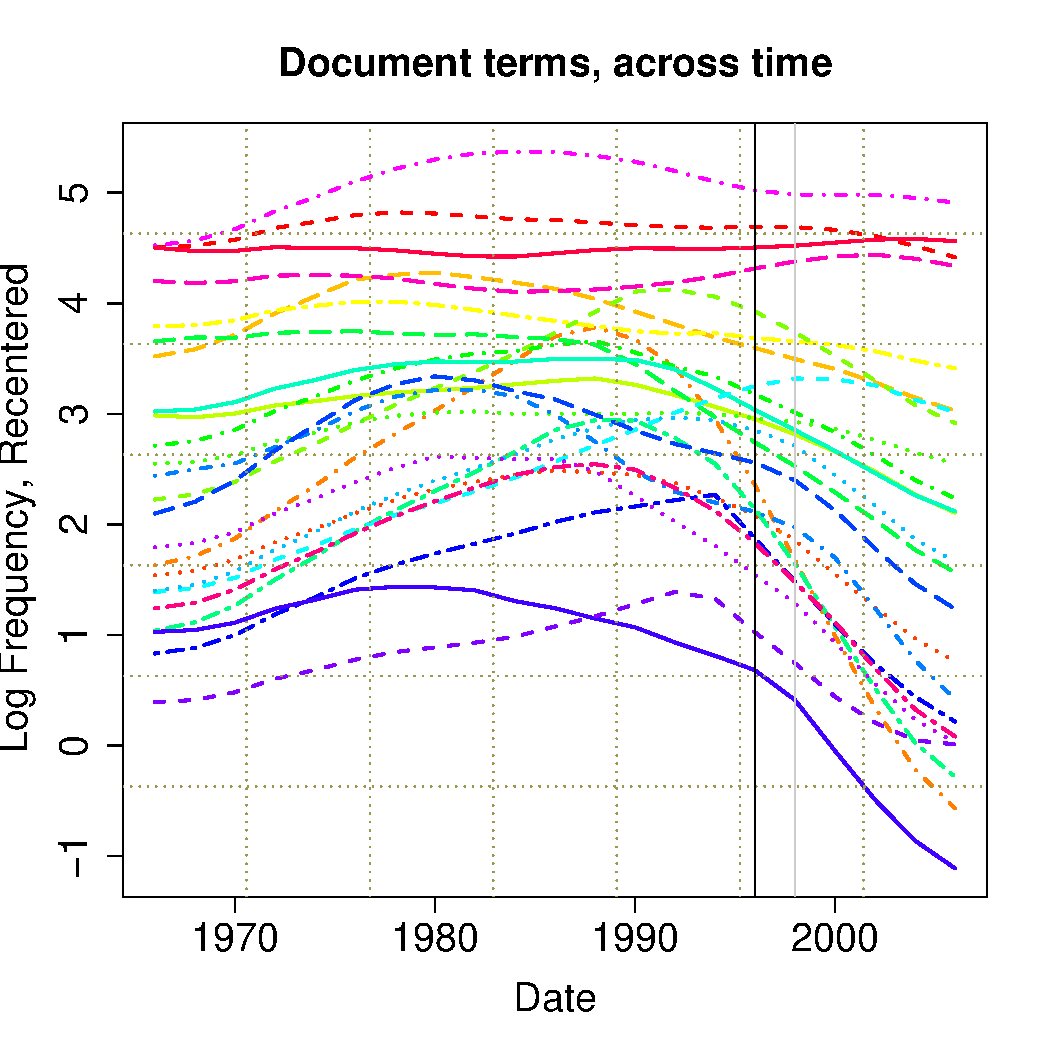
\includegraphics[width=0.3\textwidth]{nips2009/C96-2118_0_terms_time.pdf} \\
% 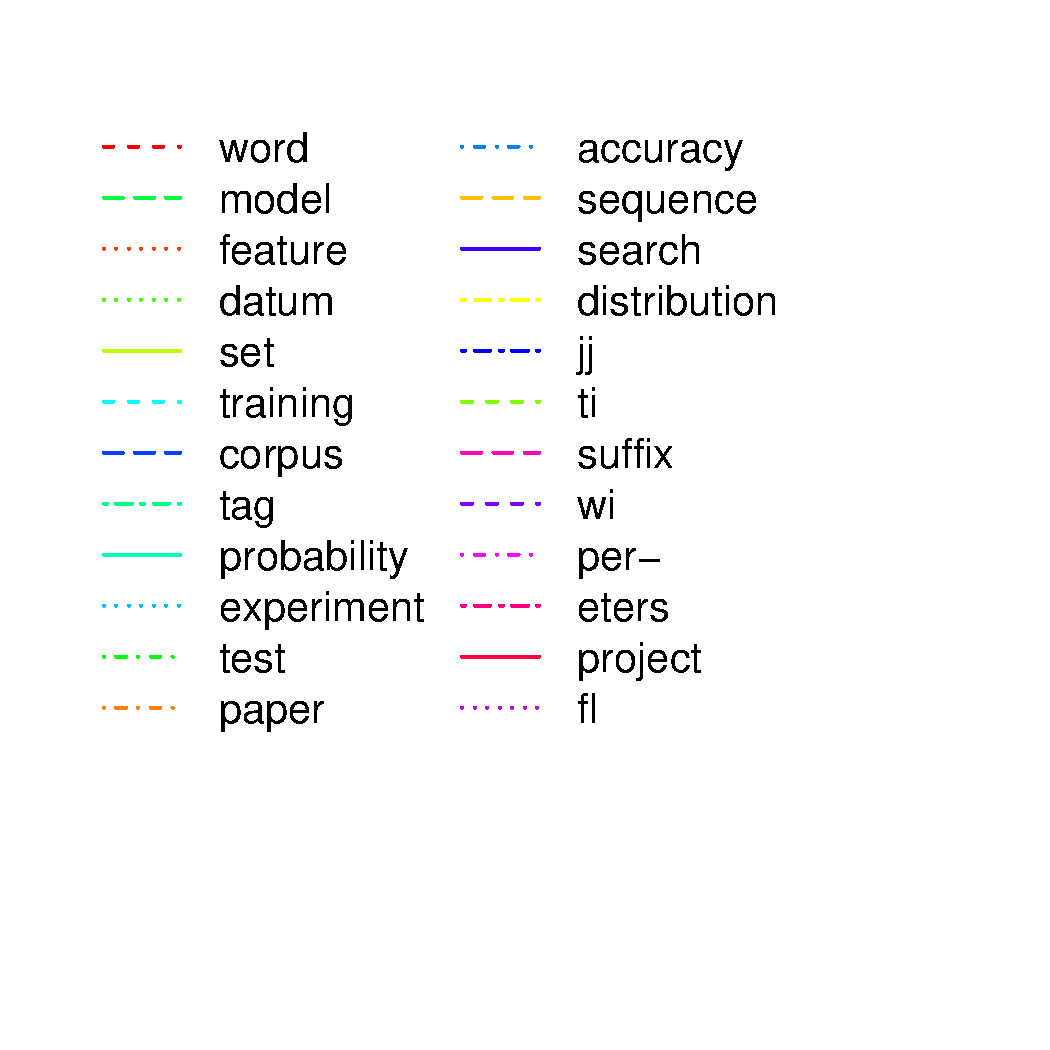
\includegraphics[width=0.3\textwidth]{nips2009/W96-0213_0_term_legend.pdf}
%      &  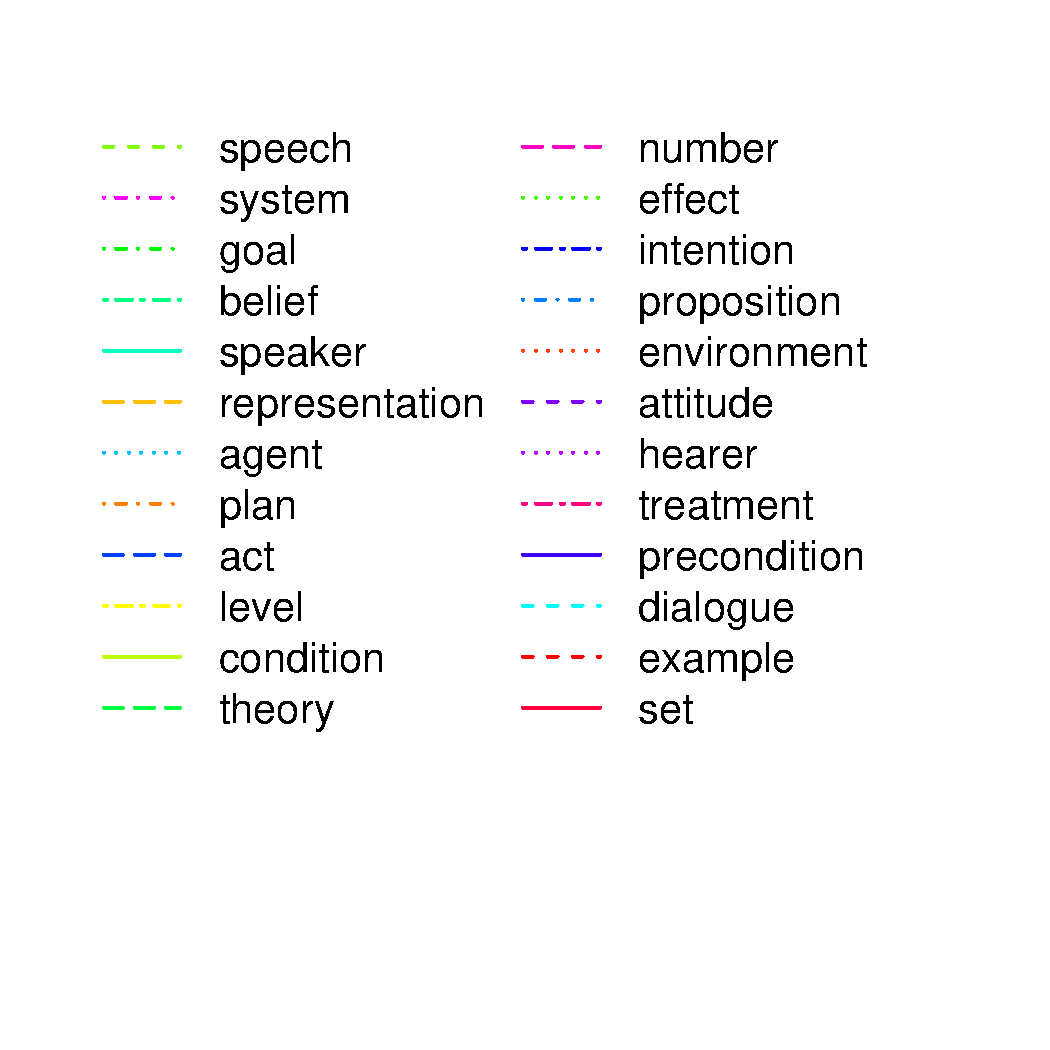
\includegraphics[width=0.3\textwidth]{nips2009/C96-2118_0_term_legend.pdf}
     \end{tabular}
      \caption{Term log-frequency within two selected topics for
        documents from \emph{The ACL} and \emph{Nature}.}
   \end{figure}
       
%}



%% \begin{figure}
%% \tiny
%% \begin{tabular}{|l|c|c|c|}
%% \hline
%% \textbf{Title} & \textbf{Year} { } { } & \textbf{Citations} & \textbf{Median}
%% \\ \hline
%% Discourse-Oriented Anaphora Resolution In Natural & & & \\ % & \\
%% Language Understanding: A Review  &  1981   &  \textbf{6}  &  1  \\ \hline %%&  6  \\ \hline
%% Natural-Language Interface  &  1982  &  \textbf{2}  &  0  \\ \hline %%&  2  \\ \hline
%% How To Parse Gaps In Spoken Utterances  &  1983    &  1  &  1  \\ \hline %%&  4  \\ \hline
%% A Stochastic Approach To Sentence Parsing  &  1984    &  \textbf{4}  &  2  \\ \hline %%&  5  \\ \hline
%% Using Restriction To Extend Parsing Algorithms For & & & \\ % & \\
%% Complex-Feature-Based Formalisms  &  1985   &  \textbf{57}  &  3  \\ \hline %%&  7  \\ \hline
%% On The Use Of Term Associations In Automatic Information Retrieval  &  1986   &  1  &  1  \\ \hline %%&  4  \\ \hline
%% Tools And Methods For Computational Lexicology  &  1987   &  \textbf{22}  &  1  \\ \hline %%&  4  \\ \hline
%% The Experience Of Developing A Large-Scale Natural Language Text & & & \\ % & \\
%% Processing System: Critique  &  1988    &  \textbf{4}  &  2  \\ \hline %%&  5  \\ \hline
%% Improvements In The Stochastic Segment Model For & & & \\ % & \\
%% Phoneme Recognition  &  1989   &  \textbf{3}  &  2  \\ \hline %%&  5  \\ \hline
%% Deducing Linguistic Structure From The Statistics Of Large Corpora  &  1990   &  \textbf{22}  &  1  \\ \hline %%&  5  \\ \hline
%% A Dynamic Language Model For Speech Recognition  &  1991  &  \textbf{11}  &  1  \\ \hline %%&  5  \\ \hline
%% Feature Selection And Feature Extract Ion For Text Categorization  &  1992   &  \textbf{3}  &  1  \\ \hline %%&  5  \\ \hline
%% HMM-Based Part-Of-Speech Tagging For Chinese Corpora  &  1993    &  \textbf{7}  &  1  \\ \hline %%&  5  \\ \hline
%% Similarity-Based Estimation Of Word Cooccurrence Probabilities  &  1994   &  \textbf{24}  &  1  \\ \hline %%&  4  \\ \hline
%% Text Chunking Using Transformation-Based Learning  &  1995   &  \textbf{143}  &  4  \\ \hline %%&  13  \\ \hline
%% A Maximum Entropy Model For Part-Of-Speech Tagging  &  1996   &  \textbf{215}  &  1  \\ \hline %%&  5  \\ \hline
%% High Performance Segmentation Of Spontaneous Speech Using & & & \\ % & \\
%% Part Of Speech And Trigger Word Information  &  1997  &  2  &  2  \\ \hline %%&  7  \\ \hline
%% Trainable, Scalable Summarization Using Robust NLP And Machine Learning  &  1998   &  \textbf{5}  &  1 \\ \hline %% &  5  \\ \hline
%% Untangling Text Data Mining  &  1999   &  \textbf{8}  &  2  \\ \hline %%&  7  \\ \hline
%% Use Of Support Vector Learning For Chunk Identification  &  2000    &  \textbf{38}  &  2  \\ \hline %%&  5  \\ \hline
%% Low-Cost, High-Performance Translation Retrieval: Dumber Is Better  &  2001   &  2  &  2  \\ \hline %%&  5  \\ \hline
%% Extracting Important Sentences With Support Vector Machines  &  2002   &  \textbf{5}  &  2  \\ \hline %%&  6  \\ \hline
%% Evaluation And Extension Of Maximum Entropy Models & & & \\ % & \\
%% With Inequality Constraints  &  2003    &  \textbf{10}  &  2  \\ \hline %%&  6  \\ \hline
%% Text Mining - Next Steps For Drug Discovery  &  2004    &  0  &  1  \\ \hline %%&  4  \\ \hline
%% A General Technique To Train Language Models On Language Models  &  2005    &  2  &  2  \\ \hline %%&  4  \\ \hline
%% %Interpreting Comparative Constructions In Biomedical Text  &  2007  &  0  &  1  &  1  &  2  \\ \hline
%% \end{tabular}

%% \label{fig:acl_influential}
%% \caption{ ACL documents with highest scores from each year
%% from 1981 to 2005.  \textbf{Splitting ties, their citations are above
%% the median 76\% of the time and in the top quartile 41\% of the time.}
%% }
%% \end{figure}
%}
      \end{block}
\end{column}

\begin{column}{.29\linewidth}
%  \vspace{4cm}
\begin{block}{Model}
%\hspace{-3.5cm} \parbox{0.93\textwidth}{

\begin{figure}
\includegraphics[width=0.8\textwidth]{../figures/docinf_gm.pdf}
\vspace{-27cm}
\caption{\small Topics $\beta$ drift over time, and documents $D$ are
generated from these topics.  At the same time, documents influence
topic drift with their words $w$ and topic-specific weights $\l$.  In
the actual model, arrows exist between nonadjacent times; we omit these for
clarity. \normalsize}
\end{figure}
\end{block}
\begin{block}{Model Notation}
%\rule[0.0cm]{26cm}{0.05cm}
\vspace{-2cm}
\small
     \begin{columns}
     \begin{column}{.45\linewidth}
     \begin{itemize}
       \item $\theta$: Topic proportion (multinomial distribution over topics)
        \item $\alpha$: Prior over topic proportions
        \item $\beta$: Topics (distributions over words)
        \item $k$: Topic ($K$ topics total)
        \item $d_t$: Document at time $t$ ($A_t$ documents at each time)
\end{itemize}
\end{column}
\begin{column}{.40\linewidth}
\begin{itemize}
        \item $\z$: Topic indicator for word
        \item $w$: Observed word
	\item $\W_s$: Term-document matrix, time s
        \item $l_{t,k}$: Influence of documents at time $t$ on topic $k$
        \item $\sigma_d^2$: variance of document weight
	\item $\sigma^2$: Topic drift variance
    \end{itemize}
\end{column}
\end{columns}
%}
\normalsize

%\vspace{1cm}
%   }

\end{block}

\begin{block}{Generative Model}
\vspace{-.9cm}
%\parbox{.95\linewidth}{ 
%\begin{columns}
%\begin{column}{.46\linewidth}

\begin{itemize}
\item  For topic $k = 1, \ldots, K$: \label{gen:beta} \\
  \begin{itemize}
  \item For time $t = 1, \ldots, T$:
    Draw $\beta_{t,k} | \beta_{t-1,k}, \z_{t-1}, l_{t-1} \sim
    \mathcal{N}(\beta_{t-1,k} + \textcolor{blue}{\mbox{Infl}(l_{t-1, k})}, \sigma^2 I)$.
  \end{itemize}
\end{itemize}
\begin{itemize}
\item  For time $t=1, \ldots, T$
  \begin{itemize}
  \item For each document $d_t$:
    \begin{itemize}
    \item Generate document $d_t$ using traditional LDA with parameters
      $\alpha$ and $\beta_{t}$.
    \item For topic $k = 1, \ldots, K$,  \label{gen:l}
      draw document weight $l_{d,k} \sim \mathcal{N}(\textbf{0}, \sigma_d^2 I)$.
    \end{itemize}
  \end{itemize}
\end{itemize}

\hspace{-2.0cm} \parbox{0.93\textwidth}{
Above is the influence function \small $\textcolor{blue}{\mbox{Infl}(l_{t-1, k}) :=
\exp(-\beta_{t-1, k}) \circ ([\z_{t-1}]_k \circ W_{t-1}) l_{t-1,k}}$ \normalsize or
\small \textcolor{blue}{$\exp(-\beta_{t-1, k}) \circ \sum_{s=1}^{t-1} r(t-s) ([\z_{s}]_k \circ W_{s})  l_{s, k}$} \normalsize
for suitable ``influence envelope'' $r(s)$. ($\circ$ denotes the element-wise
 Hadamard product, and $[z]_k$ the indicator describing whether term $z$ is in topic $k$.)
}
\end{block}
%\end{column}
%\begin{column}{.46\linewidth}
%  \end{column}
%  \end{columns}
%}
%\normalsize

%}

%%%%%%%%%%%%%%%%%%%%%%%%%%%%%%%%%%%%%%%%%%%%%%%%%%%%%%%%%%%%%%%%%%%%%%%%%%%%%%%%%%%%%%%%%%%%%%%%%%%%%%%%%%%%
 %%%%%%%%%%%%%%%%%%%%%%%%%%%%%%%%%%%%%%%%%%%%%%%%%%%%%%%%%%%%%%%%%%%%%%%%%%%%%%%%%%%%%%%%%%%%%%%%%%%%%%%%%%%%
    \end{column}

   %%%%%%%%%%%%%%%%%%%%%%%%%%%%%%%
    
    \begin{column}{.32\linewidth}

\begin{block}{Inference}
\hspace{-1.8cm} \parbox{0.93\textwidth}{
We use structured variational inference to approximate the posterior.
Inference is similar to the Dynamic Topic Model, with an additional
variational parameter for each document's influence which factorizes with
the rest of the variational posterior.  The update equation for
document weights is a key piece of this model; it is a
linear regression for each time $t$, which falls directly out of the generative model.
}
  \end{block}

\begin{block}{Results}
\hspace{-1.8cm} \parbox{.93\textwidth} { We verified the relationship
  between the posterior influence and academic citation count (a
  standard notion of bibliometric impact) for varying numbers of
  topics on subsets of three corpora:
\begin{itemize}
  \item \emph{The Association for Computational Linguistics Anthology} (7,561 docs)
  \item \emph{Proceedings of the National Academy of Sciences} (12,145 docs)
  \item \emph{Nature} (34,418 docs)
\end{itemize}
We found a statistically significant relationship between posterior
influence and citation.  We also developed a single-topic heuristic
which performs similarly well (better for PNAS; worse for ACL and
Nature).
\center{
\begin{figure}
\begin{tabular}{c}
  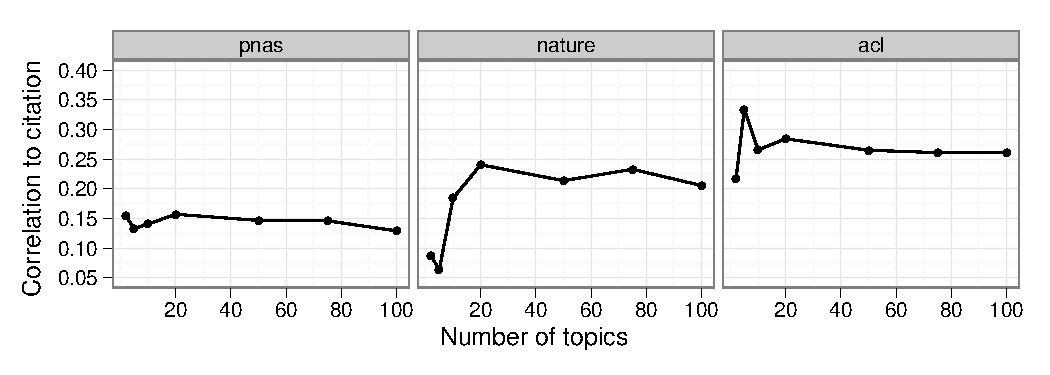
\includegraphics[width=0.9\textwidth]{../figures/results_correlation.pdf} \\
  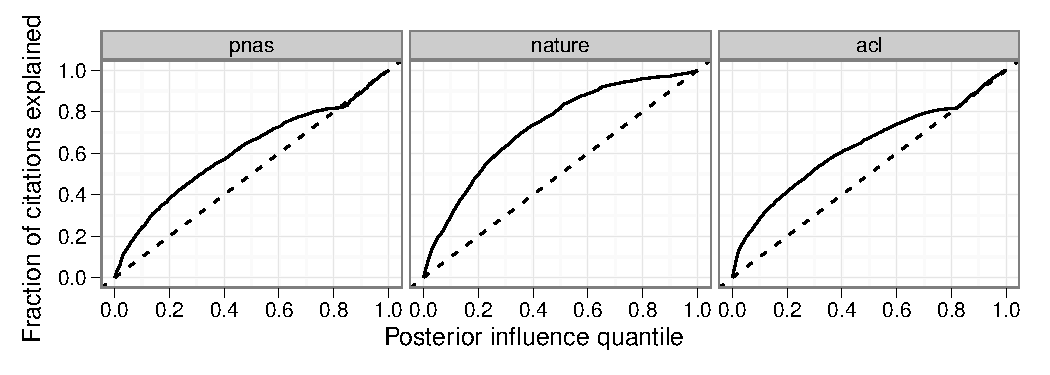
\includegraphics[width=0.9\textwidth]{../figures/results_roc.pdf}
\end{tabular}
\end{figure}
}
}
\end{block}



\begin{block}{Future Research Directions}
\hspace{-1.8cm} \parbox{.93\textwidth}{
Some areas for improvement and future research?

  \begin{itemize}
    \item Enforce a nonnegative prior over influence
    \item Explore other models
    \begin{itemize}
       \item Model topics with birth / death and forking processes
       \item Understand inter-document influence
       \item Track document influence of Dirichlet parameters $\alpha$
    \end{itemize} 
    \item Understand ground truth better
    \begin{itemize}
      \item Online behavior: ``usage'' of articles by researchers
      \item Understand cases when established metrics differ from our metric
   \end{itemize}
  \end{itemize}
}
\end{block}


    \end{column}
 \end{columns}

\end{frame}


\end{document}


%%%%%%%%%%%%%%%%%%%%%%%%%%%%%%%%%%%%%%%%%%%%%%%%%%%%%%%%%%%%%%%%%%%%%%%%%%%%%%%%%%%%%%%%%%%%%%%%%%%%
%%% Local Variables: 
%%% mode: latex
%%% TeX-PDF-mode: t
%%% End: 
